%% ============================================================
%%  Adaptive Neural Control for Mars Rover Wheel Entrapment
%%  Recovery in Granular Terrain
%%
%%  Target: IEEE Transactions on Robotics / IROS 2026
%%  Authors: Meraj Hossain Promit, Chandak Chakma
%%  Supervisors: Md. Jubair Ahmed Sourov, Dr. Sejuti Rahman
%%  University of Dhaka — Dept. Robotics & Mechatronics Engineering
%% ============================================================

\documentclass[conference]{IEEEtran}

\usepackage[utf8]{inputenc}
\usepackage[T1]{fontenc}
\usepackage{microtype}
\usepackage{amsmath,amssymb,bm}
\usepackage{graphicx}
\graphicspath{{../experiments/regolith_recovery/plots/}{figures/}}
\usepackage{booktabs}
\usepackage{array}
\usepackage{tabularx}
\usepackage{multirow}
\usepackage{subcaption}
\usepackage{hyperref}
\usepackage{xcolor}
\usepackage{cite}
\usepackage{algorithm}
\usepackage{algpseudocode}
\usepackage{float}
\usepackage{balance}
\usepackage{placeins}
\usepackage{tikz}
\usetikzlibrary{shapes.geometric,arrows.meta,positioning,calc,
                fit,backgrounds,chains}
\usepackage{fontawesome5}

\hypersetup{colorlinks=true,linkcolor=blue,citecolor=blue,urlcolor=blue}

%% ── Colours ──────────────────────────────────────────────────────────────────
\definecolor{marsred}{RGB}{150,40,20}
\definecolor{deepblue}{RGB}{40,60,100}
\definecolor{boxgray}{RGB}{248,248,248}
\definecolor{headerblue}{RGB}{50,80,130}
\definecolor{accentorange}{RGB}{200,100,30}
\definecolor{softgreen}{RGB}{60,140,60}
\definecolor{softpurple}{RGB}{100,60,150}
\definecolor{softcyan}{RGB}{40,130,150}
\definecolor{lightblue}{RGB}{220,235,250}
\definecolor{lightorange}{RGB}{255,235,210}
\definecolor{lightred}{RGB}{255,220,220}
\definecolor{lightgreen}{RGB}{220,245,220}
\definecolor{MarsRust}{HTML}{C1440E}
\definecolor{ArcticTeal}{HTML}{00897B}
\definecolor{AccentGreen}{HTML}{2E7D32}
\definecolor{WarnOrange}{HTML}{E65100}
\definecolor{SandGold}{HTML}{A67C00}
\definecolor{NebulaPurple}{HTML}{4A3F8C}
\definecolor{CosmicBlue}{HTML}{E9ECEF}
\definecolor{TextLight}{HTML}{2D3748}
\definecolor{CardBg}{HTML}{F4F6F9}
\definecolor{DimText}{HTML}{6C757D}
\definecolor{StarWhite}{HTML}{111111}

% ══════════════════════════════════════════════════════════════
\begin{document}

\title{Adaptive Neural Control for Mars Rover\\
       Wheel Entrapment Recovery in Granular Terrain}

\author{%
  \IEEEauthorblockN{Meraj Hossain Promit\IEEEauthorrefmark{1},
                    Chandak Chakma\IEEEauthorrefmark{1}}
  \IEEEauthorblockA{%
    \IEEEauthorrefmark{1}Department of Robotics and Mechatronics Engineering\\
    University of Dhaka, Dhaka, Bangladesh\\
    \{merajhossainpromit, chandakchakma\}@du.ac.bd}
  \and
  \IEEEauthorblockN{Md.~Jubair Ahmed Sourov\IEEEauthorrefmark{2},
                    Dr.~Sejuti Rahman\IEEEauthorrefmark{2}}
  \IEEEauthorblockA{%
    \IEEEauthorrefmark{2}Department of Robotics and Mechatronics Engineering\\
    University of Dhaka, Dhaka, Bangladesh}
}

\maketitle

% ── Abstract ─────────────────────────────────────────────────────────────────
\begin{abstract}
Wheel entrapment in granular regolith is one of the most critical failure modes
for planetary rovers, as demonstrated by the permanent loss of NASA's Spirit rover
in 2009. We present an autonomous entrapment recovery system for a 6-wheel
rocker-bogie Mars rover trained entirely in simulation using deep reinforcement
learning (DRL). Our primary contribution is the first coupling of Newton Material
Point Method (MPM) granular physics with MuJoCo rigid-body dynamics inside Isaac
Lab's DirectRLEnv for RL-based entrapment recovery, producing physically accurate
wheel--soil interaction under Martian gravity ($3.72\,\text{m/s}^2$). A recurrent
policy (PPO + GRU, hidden size 256) with an asymmetric critic --- actor observes
a 29-dimensional proprioceptive vector, critic additionally reads 8 privileged
simulator features --- is trained for 200\,000 timesteps across 32 parallel
environments on a single workstation with an NVIDIA RTX 5070\,Ti. The policy is
validated in a sim-to-sim A$\to$B navigation scenario: the escape primitive is
activated by a dual-mode entrapment detector and, upon completion, control returns
to a PD navigation brain. Final escape and goal-reach rates are reported in
Table~\ref{tab:results} and Table~\ref{tab:sim2sim}. The policy develops emergent
escape behaviours including coordinated rocking manoeuvres and asymmetric
wheel-steering sequences. To our knowledge, this is the first DRL-based
entrapment recovery system to employ full granular MPM coupling for a rocker-bogie
platform under Mars gravity, and the first to demonstrate zero-shot goal-directed
recovery through omnidirectional heading generalisation.
\end{abstract}

\begin{IEEEkeywords}
planetary rovers, wheel entrapment, reinforcement learning, granular simulation,
Material Point Method, PPO, GRU, Mars, regolith, curriculum learning,
sim-to-sim validation, dual-brain architecture
\end{IEEEkeywords}

% ══════════════════════════════════════════════════════════════
\section{Introduction}
\label{sec:intro}

On May~1, 2009, NASA's Spirit rover drove into soft sulfate-rich regolith and
never moved again~\cite{arvidson2011spirit}. Eight months of carefully scripted
extraction commands, constrained by a 4--24 minute round-trip communication delay,
failed to free the vehicle. Spirit had no on-board capability to detect or respond
to the entrapment autonomously---\emph{it had no way to save itself}.

Wheel entrapment in granular regolith is a systemic risk for Mars exploration.
Rovers operate over extensive dune fields, impact crater interiors filled with
fine regolith, and wind-blown sand deposits. The rocker-bogie suspension, while
excellent on rocky terrain, can cause individual wheels to sink disproportionately
in loose material. As missions extend beyond planned durations---Spirit operated
for $5\times$ its planned 90-sol lifetime, Opportunity for $55\times$---the
probability of encountering entrapment-prone terrain grows monotonically.

The fundamental operational constraint is autonomy: one-way communication
latencies of up to 24 minutes make real-time teleoperation impossible during
entrapment events. Any practical recovery system must operate entirely on-board,
detecting entrapment and executing recovery manoeuvres without ground intervention.

Prior DRL-based recovery work~\cite{bi2026escape,jain2019} addresses either
4-wheel skid-steered platforms in rigid terrain or simplified soil models. No
existing method trains a recovery policy for a \emph{6-wheel rocker-bogie rover}
in \emph{physics-accurate granular simulation} under \emph{Mars gravity}. These
three factors jointly determine the problem's difficulty: granular sinkage
progresses over several seconds (requiring memory), Mars gravity reduces
wheel--soil traction by 62\%, and rocker-bogie kinematics create coupled sinkage
dynamics across axles that demand a larger, more expressive action space.

\begin{figure*}[t]
  \centering
  \resizebox{0.92\textwidth}{!}{%
    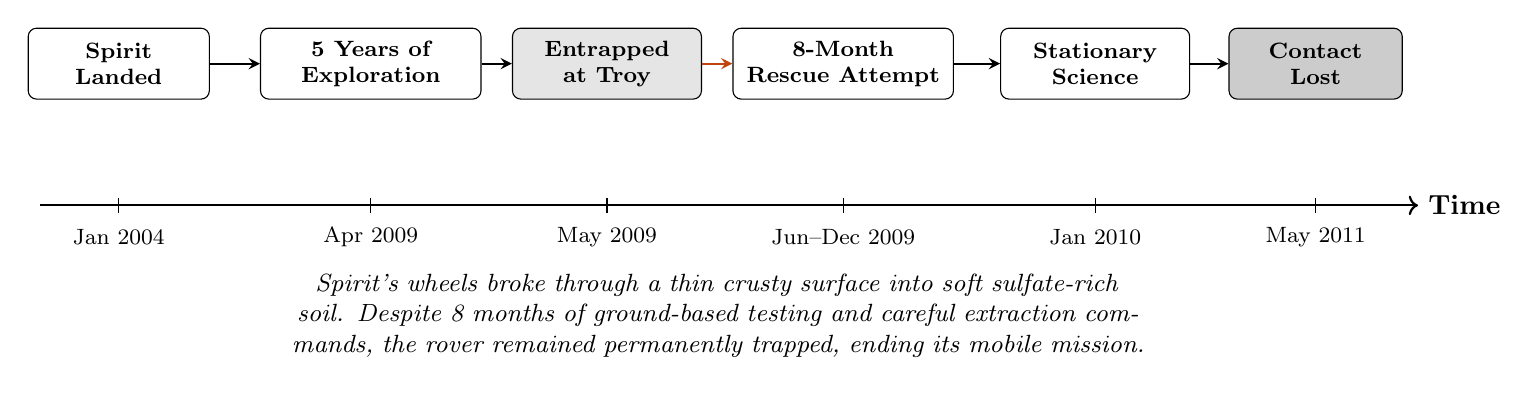
\begin{tikzpicture}[
      box/.style={rectangle, rounded corners=3pt, draw=black, fill=white,
                  minimum height=0.9cm, align=center, font=\footnotesize\bfseries},
      arrow/.style={->, >=stealth, thick}
    ]
      \node[box, minimum width=2.3cm] (b1) at (0,0)    {Spirit\\Landed};
      \node[box, minimum width=2.8cm] (b2) at (3.2,0)  {5 Years of\\Exploration};
      \node[box, minimum width=2.4cm, fill=gray!20] (b3) at (6.2,0)  {Entrapped\\at Troy};
      \node[box, minimum width=2.8cm] (b4) at (9.2,0)  {8-Month\\Rescue Attempt};
      \node[box, minimum width=2.4cm] (b5) at (12.4,0) {Stationary\\Science};
      \node[box, minimum width=2.2cm, fill=gray!40] (b6) at (15.2,0) {Contact\\Lost};
      \draw[arrow] (b1)--(b2);
      \draw[arrow] (b2)--(b3);
      \draw[arrow, color=MarsRust] (b3)--(b4);
      \draw[arrow] (b4)--(b5);
      \draw[arrow] (b5)--(b6);
      \draw[->, thick] (-1,-1.8)--(16.5,-1.8) node[right]{\textbf{Time}};
      \foreach \x/\lbl in {0/Jan 2004, 3.2/Apr 2009, 6.2/May 2009,
                            9.2/Jun--Dec 2009, 12.4/Jan 2010, 15.2/May 2011}{
        \draw (\x,-1.7)--(\x,-1.9);
        \node[font=\footnotesize] at (\x,-2.2) {\lbl};
      }
      \node[text width=15cm, align=center, font=\small\itshape] at (7.6,-3.2) {%
        Spirit's wheels broke through a thin crusty surface into soft sulfate-rich
        soil. Despite 8 months of ground-based testing and careful extraction
        commands, the rover remained permanently trapped, ending its mobile mission.};
    \end{tikzpicture}%
  }
  \caption{Timeline of the Spirit rover entrapment incident. After 5 years of
    successful exploration, Spirit became permanently immobilised at site ``Troy''
    in May~2009. The rover had no autonomous detection or recovery capability.
    This work builds the autonomy Spirit never had.}
  \label{fig:spirit_timeline}
\end{figure*}

\textbf{Contributions:}
\begin{enumerate}
  \item First coupling of Newton MPM granular physics with MuJoCo rigid-body
        dynamics inside Isaac Lab's DirectRLEnv for DRL-based entrapment recovery
        on a rocker-bogie platform under Mars gravity.
  \item Recurrent PPO+GRU policy with asymmetric actor-critic (29D actor,
        37D privileged critic), dual entrapment detection combining slip-ratio
        and torque anomaly, and an 8-term shaped reward that elicits emergent
        rocking and asymmetric-steer escape strategies.
  \item Omnidirectional escape generalisation: training with per-episode uniformly
        random headings enables \emph{zero-shot} GPS-directed escape at deployment
        without any heading-specific fine-tuning.
  \item Sim-to-sim A$\to$B navigation validation using a dual-brain architecture
        (PD navigation~$\to$~entrapment detection~$\to$~PPO recovery~$\to$~re-plan),
        with quantitative comparison against a no-recovery baseline.
\end{enumerate}

% ══════════════════════════════════════════════════════════════
%  FULL-WIDTH FIGURE: System Overview  (two-column)
% ══════════════════════════════════════════════════════════════
\begin{figure*}[t]
  \centering
  \resizebox{0.86\textwidth}{!}{%
    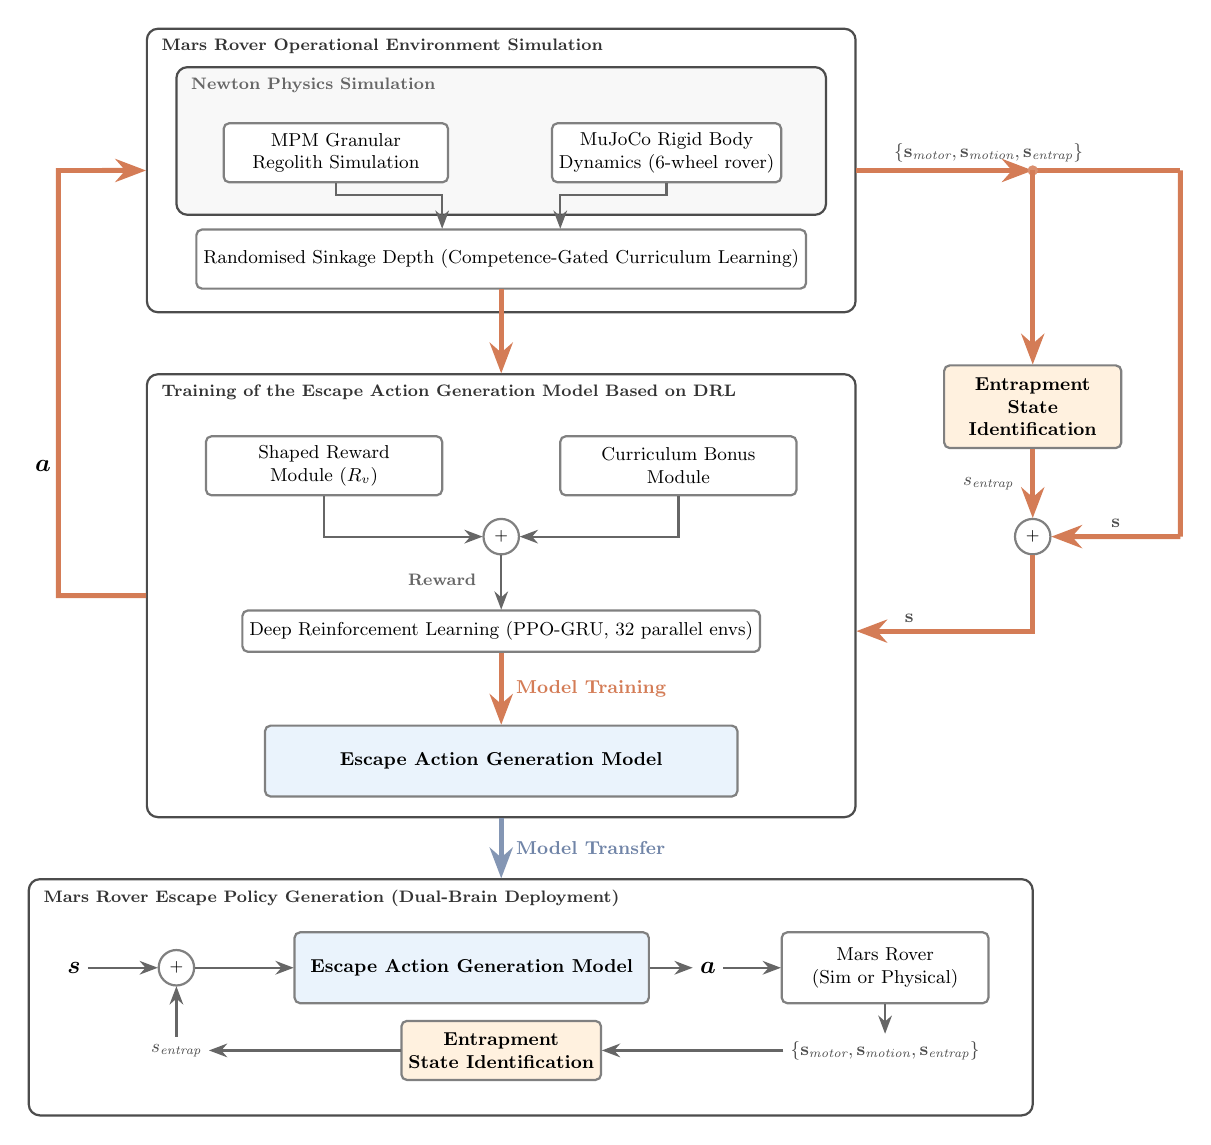
\begin{tikzpicture}[
      scale=0.75, transform shape,
      outerbox/.style={rectangle, draw=black!70, thick, rounded corners=4pt,
                       inner sep=10pt},
      innerbox/.style={rectangle, draw=black!50, thick, fill=white,
                       minimum height=1cm, minimum width=3.8cm,
                       align=center, font=\small, rounded corners=2pt},
      orangebox/.style={innerbox, fill=lightorange!70, font=\small\bfseries},
      bluebox/.style={innerbox, fill=lightblue!60, font=\small\bfseries},
      redarrow/.style={-Stealth, line width=1.8pt, color=MarsRust!70},
      bluearrow/.style={-Stealth, line width=1.8pt, color=headerblue!60},
      arrow/.style={-Stealth, thick, color=black!60},
      circnode/.style={draw=black!50, circle, thick, minimum size=0.6cm,
                       inner sep=0pt, font=\footnotesize},
      every node/.style={font=\small}
    ]
      %% Training environment block
      \node[outerbox, fill=white, minimum width=12cm, minimum height=4.8cm]
            (simbox) at (0, 12.5) {};
      \node[font=\footnotesize\bfseries, anchor=north west, text=black!80]
            at ([xshift=4pt, yshift=-2pt]simbox.north west)
            {Mars Rover Operational Environment Simulation};
      \node[outerbox, fill=boxgray, minimum width=11cm, minimum height=2.5cm]
            (physbox) at (0, 13.0) {};
      \node[font=\footnotesize\bfseries, anchor=north west, text=black!60]
            at ([xshift=4pt, yshift=-2pt]physbox.north west)
            {Newton Physics Simulation};
      \node[innerbox] (mpm)   at (-2.8, 12.8) {MPM Granular\\Regolith Simulation};
      \node[innerbox] (rigid) at ( 2.8, 12.8) {MuJoCo Rigid Body\\Dynamics (6-wheel rover)};
      \node[innerbox, minimum width=7cm] (terrain) at (0, 11.0)
            {Randomised Sinkage Depth (Competence-Gated Curriculum Learning)};
      %% Entrapment identifier
      \node[orangebox, minimum width=3cm, minimum height=1.4cm]
            (entrapid) at (9, 8.5) {\textbf{Entrapment}\\State\\Identification};
      %% Training block
      \node[outerbox, fill=white, minimum width=12cm, minimum height=7.5cm]
            (trainbox) at (0, 5.3) {};
      \node[font=\footnotesize\bfseries, anchor=north west, text=black!80]
            at ([xshift=4pt, yshift=-2pt]trainbox.north west)
            {Training of the Escape Action Generation Model Based on DRL};
      \node[innerbox, minimum width=4cm] (handrew)  at (-3, 7.5)
            {Shaped Reward\\Module ($R_v$)};
      \node[innerbox, minimum width=4cm] (curricrew) at (3, 7.5)
            {Curriculum Bonus\\Module};
      \node[circnode] (plus) at (0, 6.3) {$+$};
      \node[below=0.2cm of plus, xshift=-1.0cm, font=\footnotesize\bfseries,
            text=black!60] {Reward};
      \node[innerbox, minimum width=8cm, minimum height=0.7cm] (drl) at (0, 4.7)
            {Deep Reinforcement Learning (PPO-GRU, 32 parallel envs)};
      \node[circnode] (sconcat) at (9, 6.3) {$+$};
      \node[font=\large\bfseries\itshape, anchor=east] (abig) at (-7.5, 7.5)
            {$\boldsymbol{a}$};
      %% Escape model box
      \node[bluebox, minimum width=8cm, minimum height=1.2cm]
            (escapemodel) at (0, 2.5) {\textbf{Escape Action Generation Model}};
      %% Physics connections
      \draw[arrow] (mpm.south)   -- ++(0,-0.2) -| ([xshift=-1cm]terrain.north);
      \draw[arrow] (rigid.south) -- ++(0,-0.2) -| ([xshift= 1cm]terrain.north);
      \draw[redarrow] (terrain.south) -- (trainbox.north);
      %% State flow
      \coordinate (split) at (9, 12.5);
      \coordinate (hTip)  at (11.5, 12.5);
      \draw[redarrow] (simbox.east) -- (split)
          node[pos=0.75, above, font=\small\itshape, text=black!70]
              {$\{\mathbf{s}_{\text{motor}}, \mathbf{s}_{\text{motion}},
                \mathbf{s}_{\text{entrap}}\}$};
      \draw[redarrow, -{}] (split) -- (hTip);
      \fill[MarsRust!60] (split) circle (2.5pt);
      \draw[redarrow] (split) -- (entrapid.north);
      \draw[redarrow] (entrapid.south) -- (sconcat.north)
          node[midway, left=5pt, font=\small\itshape, text=black!70]
              {$s_{\text{entrap}}$};
      \draw[redarrow, -{}] (hTip) -- (11.5, 6.3);
      \draw[redarrow] (11.5, 6.3) -- (sconcat.east)
          node[midway, above, font=\small\itshape, text=black!70]
              {$\mathbf{s}$};
      \draw[redarrow] (sconcat.south) -- (sconcat.south |- drl)
                      -- (trainbox.east |- drl)
          node[pos=0.7, above, font=\small\itshape, text=black!70] {$\mathbf{s}$};
      \draw[arrow] (handrew.south)  |- (plus.west);
      \draw[arrow] (curricrew.south) |- (plus.east);
      \draw[arrow] (plus.south) -- (drl.north);
      \draw[redarrow] (trainbox.west) -- (-7.5, 5.3)
                      -- (-7.5, 12.5) -- (simbox.west);
      \draw[redarrow] (drl.south) -- (escapemodel.north)
          node[midway, right=3pt, font=\small\bfseries, text=MarsRust!70]
              {Model Training};
      %% Deployment block
      \node[outerbox, fill=white, minimum width=17cm, minimum height=4cm]
            (deploybox) at (0.5, -1.5) {};
      \node[font=\footnotesize\bfseries, anchor=north west, text=black!80]
            at ([xshift=4pt, yshift=-2pt]deploybox.north west)
            {Mars Rover Escape Policy Generation (Dual-Brain Deployment)};
      \node[circnode] (sconcat2) at (-5.5, -1.0) {$+$};
      \node[font=\large\bfseries\itshape, anchor=east] (slbl2)
            at (-7.0, -1.0) {$\boldsymbol{s}$};
      \node[bluebox, minimum width=6cm, minimum height=1.2cm]
            (escapemodel2) at (-0.5, -1.0) {\textbf{Escape Action Generation Model}};
      \node[font=\large\bfseries\itshape] (abig2) at (3.5, -1.0) {$\boldsymbol{a}$};
      \node[innerbox, minimum width=3.5cm, minimum height=1.2cm]
            (physical) at (6.5, -1.0) {Mars Rover\\(Sim or Physical)};
      \node[orangebox, minimum width=3cm, minimum height=1cm]
            (entrapid2) at (0, -2.4) {\textbf{Entrapment}\\State Identification};
      \node[font=\small\itshape, text=black!70]
            (sabn2)     at (-5.5, -2.4) {$s_{\text{entrap}}$};
      \node[font=\small\itshape, text=black!70]
            (stateout2) at ( 6.5, -2.4)
            {$\{\mathbf{s}_{\text{motor}}, \mathbf{s}_{\text{motion}},
              \mathbf{s}_{\text{entrap}}\}$};
      \draw[bluearrow] (trainbox.south) -- (trainbox.south |- deploybox.north)
          node[midway, right=3pt, font=\small\bfseries, text=headerblue!70]
              {Model Transfer};
      \draw[arrow] (slbl2.east)      -- (sconcat2.west);
      \draw[arrow] (sabn2.north)     -- (sconcat2.south);
      \draw[arrow] (sconcat2.east)   -- (escapemodel2.west);
      \draw[arrow] (escapemodel2.east) -- (abig2.west);
      \draw[arrow] (abig2.east)      -- (physical.west);
      \draw[arrow] (physical.south)  -- (stateout2.north);
      \draw[arrow] (stateout2.west)  -- (entrapid2.east);
      \draw[arrow] (entrapid2.west)  -- (sabn2.east);
    \end{tikzpicture}%
  }
  \caption{System overview. \emph{Top:} training pipeline --- Newton MPM +
    MuJoCo simulation with competence-gated curriculum sinkage scheduling feeds an
    8-term shaped reward and curriculum bonus into PPO-GRU across 32 parallel
    environments, producing the escape action generation model.
    \emph{Bottom:} dual-brain deployment loop --- the trained model runs on the
    rover with on-board entrapment state identification; control hands off from
    the navigation brain to the escape brain and back autonomously.}
  \label{fig:system_overview}
\end{figure*}

% ══════════════════════════════════════════════════════════════
\section{Related Work}
\label{sec:related}

\subsection{Entrapment and Recovery for Wheeled Robots}

Bi and Ding~\cite{bi2026escape} is the most directly relevant prior work.
They train a PPO+LSTM policy for escape of a 4-wheel skid-steered mobile robot
(SSMR) using GAIL-fused rewards ($R = 0.9R_H + 0.1R_D$) and domain
randomisation over 20+ parameters, achieving 90\% escape success in both Unity
simulation and real-world orchard field tests. However, their system
(i)~uses rigid terrain, (ii)~operates under Earth gravity,
(iii)~targets a 4-wheel 2D action space ($\omega_l, \omega_r$), and
(iv)~requires expert demonstrations for GAIL. Our work addresses all four limitations.

Inotsume et al.~\cite{inotsume2020} demonstrate real-time slip prediction for
planetary rovers via Kalman-filter-based terramechanics estimation, focusing on
detection without active recovery. Ding et al.~\cite{ding2011} provide analytical
wheel--soil interaction models grounded in Bekker--Wong theory~\cite{bekker1960}
but without RL-based recovery. Fankhauser et al.~\cite{fankhauser2018} demonstrate multi-phase recovery for
the ANYmal quadruped (detect~$\to$ recover~$\to$ resume), providing an
architectural template that motivates our dual-brain hierarchy. Hwangbo et
al.~\cite{hwangbo2019anymal} and Lee et al.~\cite{lee2020quadruped} show that
recurrent policies trained in simulation transfer to real legged robots over
challenging terrain, motivating our GRU-based approach.

\subsection{Granular Physics Simulation for Robotics}

MPM~\cite{sulsky1994particle} is a hybrid Eulerian--Lagrangian continuum method
that correctly models sinkage progression, bulldozing resistance, and particle
redistribution during wheel spinning---phenomena invisible to rigid-body terrain
approximations. Klar et al.~\cite{klar2016sand} extended MPM to granular sand
via the Drucker--Prager yield surface, enabling realistic plastic flow in
wheel--soil contact. Stomakhin et al.~\cite{stomakhin2013snow} established the
numerical framework later adapted for sand. Bekker--Wong
terramechanics~\cite{bekker1960} provides classical analytical predictions for
wheel--soil interaction but is limited to steady-state homogeneous conditions;
MPM captures transient sinkage dynamics critical for entrapment.

\subsection{Research Gaps}

No prior DRL-based recovery work: (1) couples a rocker-bogie rover with MPM
granular physics; (2) operates under Mars gravity; (3) exploits a 10D
independent per-wheel drive-and-steer action space; (4) applies
competence-gated curriculum sinkage scheduling; or (5) demonstrates zero-shot
goal-directed escape via omnidirectional heading generalisation.

% ══════════════════════════════════════════════════════════════
\section{Problem Formulation}
\label{sec:problem}

\subsection{Entrapment Definition}

Wheel entrapment is formally characterised by the conjunction:
\begin{equation}
  f_{\text{ent}} = 1 \;\iff\;
  \begin{cases}
    |v_x| < 0.15\;\text{m/s}\\[2pt]
    \bar{\sigma}_{\text{slip}} > 0.4 \\[2pt]
    \text{both held} \geq 15\;\text{steps (0.6\,s)}
  \end{cases}
  \label{eq:entrapment}
\end{equation}
where $v_x$ is body-frame forward velocity and
$\bar{\sigma}_{\text{slip}} = \tfrac{1}{6}\sum_i(1 - v_{\text{lin},i}/\omega_i r)$
is mean slip ratio across six drive wheels. The 15-step persistence window (0.6\,s at 25\,Hz) prevents transient bumps from
triggering the flag while remaining responsive to genuine sinkage, which develops
over 2--5 seconds of wheel spinning in soft regolith.

\subsection{POMDP Formulation}

The recovery problem is a partially observable MDP. At each timestep $t$, the
rover receives observation $\mathbf{o}_t \in \mathbb{R}^{29}$ and selects action
$\mathbf{a}_t \in \mathbb{R}^{10}$ to maximise:
\begin{equation}
  J(\pi_\theta) = \mathbb{E}_{\tau \sim \pi_\theta}
  \!\left[ \sum_{t=0}^{T} \gamma^t R(\mathbf{s}_t, \mathbf{a}_t) \right],
  \quad \gamma = 0.99
  \label{eq:objective}
\end{equation}
Partial observability arises because per-wheel sinkage depth, terrain composition,
and entrapment zone boundary are not directly observable. This motivates the GRU
recurrent policy~\cite{cho2014gru}, whose hidden state $\mathbf{h}_t$ implicitly
integrates these variables from observation history. During training we exploit an asymmetric actor-critic: the critic receives an
augmented 37-dimensional observation that appends 8 privileged simulator features
(true sinkage depth, wheel burial ratio, sand-force proxy, 3D body linear
velocity, yaw rate, chassis height) on top of the 29D onboard slice. The actor
observes only the 29D slice, so the deployed controller is a pure POMDP solver
while the value head enjoys lower-variance targets.

\subsubsection{Observation Space (29D)}
\begin{equation*}
  \mathbf{o}_t = \bigl[\underbrace{\boldsymbol{\omega}_w}_{6},\;
                        \underbrace{\boldsymbol{\sigma}}_{6},\;
                        \underbrace{\mathbf{q}_{\text{steer}}}_{4},\;
                        \underbrace{\mathbf{a}_{\text{imu}}}_{3},\;
                        \underbrace{g_z}_{1},\;
                        \underbrace{\boldsymbol{\tau}}_{6},\;
                        \underbrace{f_{\text{ent}}}_{1},\;
                        \underbrace{f_{\text{anom}}}_{1},\;
                        \underbrace{x_{\text{disp}}}_{1}\bigr]
\end{equation*}
where $\boldsymbol{\omega}_w$ are normalised wheel velocities, $\boldsymbol{\sigma}$
per-wheel slip ratios, $\mathbf{q}_{\text{steer}}$ steer joint angles,
$\mathbf{a}_{\text{imu}}$ IMU linear accelerations, $g_z$ projected gravity,
$\boldsymbol{\tau}$ normalised drive torques (inspired by~\cite{bi2026escape}),
$f_\text{ent}$ the entrapment flag, $f_\text{anom}$ the torque anomaly flag, and
$x_\text{disp} = d/d_\text{esc} \in [0,1]$ the fraction of escape distance
covered.

\subsubsection{Action Space (10D)}

$\mathbf{a}_t = [\dot{\theta}_{\text{drive}} \in [-6,6]\,\text{rad/s}^6,\;
\theta_{\text{steer}} \in [-0.6,0.6]\,\text{rad}^4]$. This 10D space enables manoeuvres---asymmetric rocking, diagonal crabbing,
coordinated steer-and-drive---impossible in the 2D skid-steer action space of
all prior recovery work.

% ══════════════════════════════════════════════════════════════
\section{System Architecture}
\label{sec:architecture}

The system overview is presented in Fig.~\ref{fig:system_overview}. Three blocks
interact: (A)~the simulation environment with two-way MPM--MuJoCo coupling and
curriculum sinkage scheduling; (B)~the DRL training loop with shaped reward and
curriculum bonus; and (C)~the deployed escape policy in the dual-brain controller.
The physics stack and the recurrent policy network are detailed in
Fig.~\ref{fig:physics_stack} and Fig.~\ref{fig:policy_arch} respectively.

\begin{figure}[t]
  \centering
  \resizebox{0.92\linewidth}{!}{%
    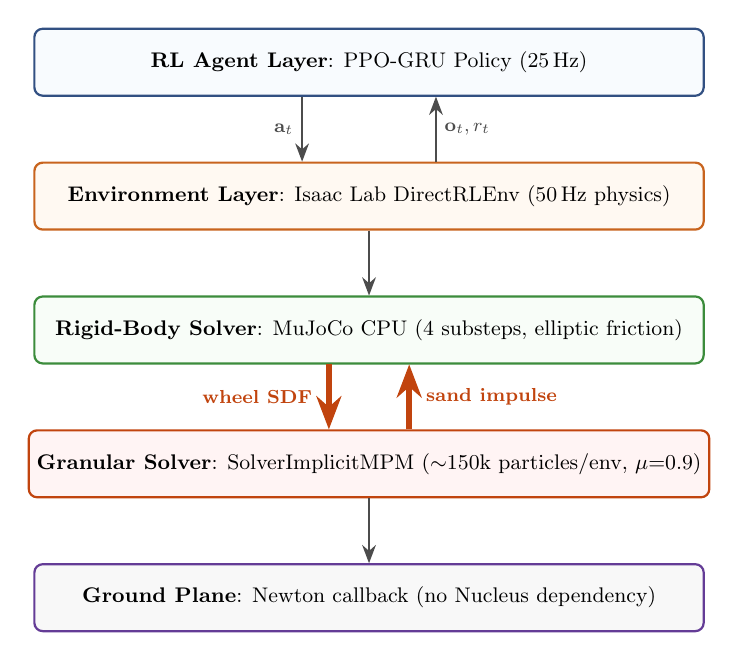
\begin{tikzpicture}[
      node distance=0.5cm,
      layer/.style={rectangle, draw=black!55, fill=white, thick, rounded corners=3pt,
                    minimum height=1.0cm, minimum width=10cm,
                    align=center, font=\small},
      arrow/.style={-Stealth, thick, color=black!70},
      scale=0.85, transform shape
    ]
      \node[layer, fill=lightblue!20, draw=headerblue] (rl) 
          at (0, 8.0)
          {\textbf{RL Agent Layer}: PPO-GRU Policy (25\,Hz)};
      \node[layer, fill=lightorange!30, draw=accentorange] (env) at (0, 6.0)
          {\textbf{Environment Layer}: Isaac Lab DirectRLEnv (50\,Hz physics)};
      \node[layer, fill=lightgreen!20, draw=softgreen] (rigid) at (0, 4.0)
          {\textbf{Rigid-Body Solver}: MuJoCo CPU (4 substeps, elliptic friction)};
      \node[layer, fill=lightred!30, draw=MarsRust] (mpm) at (0, 2.0)
          {\textbf{Granular Solver}: SolverImplicitMPM (${\sim}150\text{k}$
           particles/env, $\mu{=}0.9$)};
      \node[layer, fill=boxgray, draw=softpurple] (ground) at (0, 0.0)
          {\textbf{Ground Plane}: Newton callback (no Nucleus dependency)};
      %% Two-way coupling annotations
      \draw[arrow, line width=2pt, color=MarsRust]
          ($(rigid.south)+(-0.6,0)$) -- ($(mpm.north)+(-0.6,0)$)
          node[midway, left=0.1cm, font=\footnotesize\bfseries, text=MarsRust]
              {wheel SDF};
      \draw[arrow, line width=2pt, color=MarsRust]
          ($(mpm.north)+(0.6,0)$) -- ($(rigid.south)+(0.6,0)$)
          node[midway, right=0.1cm, font=\footnotesize\bfseries, text=MarsRust]
              {sand impulse};
      %% RL--env flow
      \draw[arrow] ($(rl.south)+(-1.0,0)$) -- ($(env.north)+(-1.0,0)$)
          node[midway, left, font=\footnotesize] {$\mathbf{a}_t$};
      \draw[arrow] ($(env.north)+(1.0,0)$) -- ($(rl.south)+(1.0,0)$)
          node[midway, right, font=\footnotesize] {$\mathbf{o}_t,r_t$};
      \draw[arrow] (env.south)  -- (rigid.north);
      \draw[arrow] (mpm.south)  -- (ground.north);
    \end{tikzpicture}%
  }
  \caption{Physics simulation stack. Two-way coupling (red arrows): wheel SDF
    geometry displaces sand particles; resulting particle impulses feed back as
    external forces on the rover body. 32 environments run in parallel, each
    with ${\sim}150$\,k MPM particles in a $3.5\times3.5\times0.3$\,m sand bed
    under Martian gravity ($g{=}3.72\,\text{m/s}^2$).}
  \label{fig:physics_stack}
\end{figure}

% ══════════════════════════════════════════════════════════════
%  FULL-WIDTH FIGURE: Per-wheel coupling  (two-column)
% ══════════════════════════════════════════════════════════════
\begin{figure*}[t]
  \centering
  \resizebox{0.82\textwidth}{!}{%
    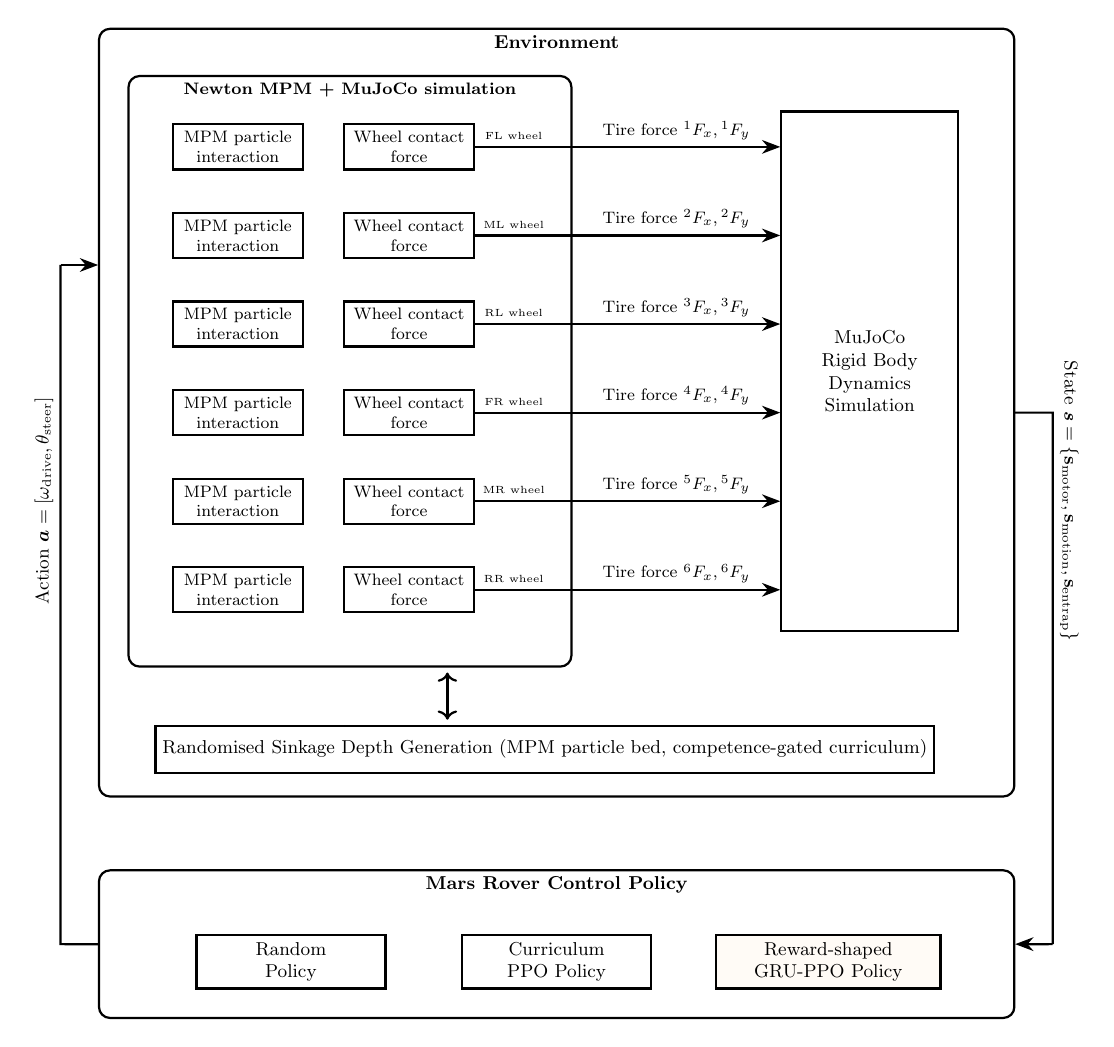
\begin{tikzpicture}[
      scale=0.75, transform shape,
      outerbox/.style={rectangle, draw=black, thick, rounded corners},
      innerbox/.style={rectangle, draw=black, thick, fill=lightblue!30,
                       minimum height=0.8cm, align=center, font=\small},
      wheelbox/.style={rectangle, draw=black, thick, fill=white,
                       minimum height=0.7cm, minimum width=2.2cm,
                       align=center, font=\footnotesize},
      arrow/.style={-Stealth, thick},
      every node/.style={font=\small}
    ]
      %% Outer Environment box
      \node[outerbox, fill=white, minimum width=15.5cm, minimum height=13cm,
            label={[font=\small\bfseries, anchor=north]north:Environment}]
            (envbox) at (0.2, 0.5) {};
      %% Inner Simulation box
      \node[outerbox, fill=white, minimum width=7.5cm, minimum height=10cm,
            label={[font=\footnotesize\bfseries, anchor=north]north:%
              Newton MPM + MuJoCo simulation}]
            (motorsim) at (-3.3, 1.2) {};
      %% Rigid body box
      \node[innerbox, minimum width=3cm, minimum height=8.8cm, fill=white]
            (rigidbody) at (5.5, 1.2)
            {MuJoCo\\Rigid Body\\Dynamics\\Simulation};
      %% 6-wheel rows
      \foreach \i/\name/\ypos in {1/FL/5, 2/ML/3.5, 3/RL/2,
                                    4/FR/0.5, 5/MR/-1, 6/RR/-2.5}{
        \node[wheelbox] (motor\i) at (-5.2, \ypos) {MPM particle\\interaction};
        \node[wheelbox] (tire\i)  at (-2.3, \ypos) {Wheel contact\\force};
        \coordinate (simright) at (motorsim.east|-tire\i.east);
        \draw[arrow] (tire\i.east) -- (rigidbody.west|-tire\i.east);
        \node[font=\tiny, anchor=south]
              at ($(tire\i.east)!0.4!(simright)$) {\name{} wheel};
        \node[font=\footnotesize, anchor=south]
              at ($(simright)!0.5!(rigidbody.west|-tire\i.east)$)
              {Tire force ${}^{\i}F_x,{}^{\i}F_y$};
      }
      %% Curriculum terrain
      \node[innerbox, minimum width=13cm, fill=white] (randterrain) at (0, -5.2)
            {Randomised Sinkage Depth Generation (MPM particle bed,
             competence-gated curriculum)};
      \coordinate (arrowpos) at ($(motorsim.south)!0.5!(randterrain.north)$);
      \draw[thick, <->] ($(arrowpos)+(0,-0.4)$) -- ($(arrowpos)+(0,0.4)$);
      %% Control policy box
      \node[outerbox, fill=white, minimum width=15.5cm, minimum height=2.5cm,
            label={[font=\small\bfseries, anchor=north]north:Mars Rover Control Policy}]
            (policybox) at (0.2, -8.5) {};
      \node[innerbox, fill=white, minimum width=3.2cm] (expert)   at (-4.3, -8.8)
            {Random\\Policy};
      \node[innerbox, fill=white, minimum width=3.2cm] (imitator) at ( 0.2, -8.8)
            {Curriculum\\PPO Policy};
      \node[innerbox, fill=lightorange!20, minimum width=3.8cm] (fusion) at (4.8, -8.8)
            {Reward-shaped\\GRU-PPO Policy};
      %% Action/state loops
      \draw[thick] (policybox.west) -- (-8.2, -8.5) -- (-8.2, 3);
      \draw[arrow] (-8.2, 3) -- (envbox.west|-{(-8.2,3)});
      \node[font=\small, rotate=90, anchor=south] at (-8.2, -1)
            {Action $\boldsymbol{a}=[\omega_\text{drive},\theta_\text{steer}]$};
      \draw[thick] (envbox.east) -- (8.6, 0.5) -- (8.6, -8.5);
      \draw[arrow] (8.6, -8.5) -- (policybox.east);
      \node[font=\small, rotate=-90, anchor=south] at (8.6, -1)
            {State $\boldsymbol{s}=\{\mathbf{s}_\text{motor},
             \mathbf{s}_\text{motion}, \mathbf{s}_\text{entrap}\}$};
    \end{tikzpicture}%
  }
  \caption{Simulation framework showing per-wheel coupling. Each of the six
    wheels produces MPM particle interaction forces and wheel contact forces, fed
    to the MuJoCo rigid-body solver as per-wheel tyre forces ${}^iF_x, {}^iF_y$.
    The control policy receives the full 29D observation and issues 10D actions
    (6 drive + 4 steer).}
  \label{fig:simulation_framework}
\end{figure*}

% ══════════════════════════════════════════════════════════════
\section{Methodology}
\label{sec:method}

\subsection{Robot Platform}

The \textit{AAU Mars Rover}~\cite{rlroverlab} is a 6-wheel rocker-bogie platform
(wheel radius $r{=}0.10$\,m) with 6 independent drive joints (velocity control,
$\pm6$\,rad/s, $\tau_{\max}{=}80$\,Nm), 4 steering joints (position control,
$\pm0.6$\,rad), and passive rocker-bogie differential joints. The simulation
couples the Newton physics engine~\cite{newton} with Isaac Lab~\cite{isaaclab}
and MuJoCo~\cite{todorov2012mujoco} as the rigid-body backend under Martian
gravity ($g{=}3.72\,\text{m/s}^2$, 62\% reduction from Earth). The drive actuators use implicit torque control (stiffness~$=0$,
damping~$=4000$\,Ns/m, effort limit~$80$\,Nm). At free-driving steady state
($v_\text{err}{\approx}0.005$\,rad/s), $\tau{\approx}20$\,Nm (ratio~$\approx0.25$).
Under burial ($v_\text{err}{\approx}2$\,rad/s), $\tau\to80$\,Nm (ratio~$=1.0$),
providing a clean binary signal for the torque anomaly detector.

\subsection{Granular Sand Simulation}

Each of the 32 parallel environments contains a $3.5{\times}3.5{\times}0.30$\,m
MPM sand bed (voxel size $0.05$\,m, PPC~$=2.0$, ${\sim}150\,000$ particles),
with friction $\mu{=}0.9$ and stiffness $k_e{=}10^{15}$\,Pa (unconditionally
stable implicit solver). The large square bed---symmetric in all
directions---ensures that omnidirectional escape training is not biased by
asymmetric runway length. The rover is spawned 0.5\,m into the bed (from the
edge in the anti-escape direction), providing $1.75+0.5+0.5{=}2.75$\,m of sand
to cross before the rear wheels clear the far edge. A 20-step settlement window after each reset ($\Delta t{=}0.02$\,s per physics
step) clamps per-body sand forces to 800\,N and torques to 80\,Nm, allowing
particles to relax around the wheels without launching the chassis under the
sudden SDF--particle overlap created by teleportation.

\subsection{Omnidirectional Escape and Zero-Shot Goal Generalisation}

Training with a fixed escape heading (e.g.~$+x$) produces a policy that can
only escape in that direction, failing when the entrapment zone lies across the
path to a GPS waypoint. Instead, at the start of each episode we sample:
\begin{equation}
  \phi_\text{esc} \sim \mathcal{U}(0, 2\pi)
\end{equation}
and orient the rover to face $\phi_\text{esc}$ (with $\pm5^\circ$ jitter). The escape direction buffer $\hat{\mathbf{e}} = [\cos\phi_\text{esc},
\sin\phi_\text{esc}]^\top$ is used in the reward, not exposed in the observation.
The result is a \emph{heading-agnostic} policy that, in the body frame, always
``escapes forward.''

At deployment, the mode-switcher sets $\hat{\mathbf{e}}$ to the direction from the
current position toward GPS goal B:
\begin{equation}
  \hat{\mathbf{e}}_\text{deploy} =
  \frac{\mathbf{p}_B - \mathbf{p}_t}{\|\mathbf{p}_B - \mathbf{p}_t\|_2}
\end{equation}
This zero-shot goal-directed recovery requires no additional training or
fine-tuning: the heading generalisation learned over $\mathcal{U}(0,2\pi)$
episodes covers every GPS bearing.

\subsection{Reward Function}

\begin{equation}
  R_t = r_{\text{prog}} + r_{\text{esc}} + r_{\text{esc,shaped}}
        + r_{\text{rock}} - p_{\text{slip}} - p_{\text{tilt}}
        - p_{\text{smooth}} - p_{\text{abn}}
  \label{eq:reward}
\end{equation}

\begin{table}[t]
  \centering
  \caption{Reward function v5 ($\Delta t{=}0.04$\,s). All terms multiply by $\Delta t$;
    the escape bonus (weight~20) dominates during entrapment. Unlike
    Bi~\&~Ding~\cite{bi2026escape}, who use GAIL-fused rewards requiring expert
    demonstrations, every term here is hand-engineered from first principles.}
  \label{tab:reward}
  \renewcommand{\arraystretch}{1.25}
  \begin{tabular}{@{}lcp{4.0cm}@{}}
    \toprule
    \textbf{Term} & \textbf{Wt.} & \textbf{Formula / Justification} \\
    \midrule
    $r_{\text{prog}}$
      & $+1.5$
      & $(\mathbf{v}_{xy} \cdot \hat{\mathbf{e}})\,\Delta t$
        — world-frame progress along escape heading \\[2pt]
    $r_{\text{esc}}$
      & $+20$
      & Milestone bonuses at 0.5, 1.0, 2.0, 3.0\,m ($\times$time scale)
        — sparse landmark rewards \\[2pt]
    $r_{\text{esc,shaped}}$
      & $+5$
      & $\Delta d \,\Delta t$ — dense distance signal between milestones \\[2pt]
    $r_{\text{rock}}$
      & $+5$
      & $\Delta v_x \cdot f_\text{ent}\,\Delta t$ — rewards rocking
        manoeuvres while trapped \\[2pt]
    $p_{\text{slip}}$
      & $-0.5$
      & $\bar{\sigma}(1{-}f_\text{ent})\,\Delta t$ — penalises spinning wheels
        during free driving only \\[2pt]
    $p_{\text{tilt}}$
      & $-0.3$
      & $\|\boldsymbol{\omega}_{xy}\|_2\,\Delta t$
        — stabilises body attitude \\[2pt]
    $p_{\text{smooth}}$
      & $-0.05$
      & $\|\mathbf{a}_t {-} \mathbf{a}_{t-1}\|_2\,\Delta t$
        — reduces high-frequency jitter \\[2pt]
    $p_{\text{abn}}$
      & $-0.3$
      & $(-v_x)^+\! f_\text{anom}(1{-}f_\text{ent})\,\Delta t$
        — penalises reversing under anomaly \\
    \bottomrule
  \end{tabular}
\end{table}

\textbf{Design rationale.}
The escape bonus weight (20) is set to ensure that a single successful
3.0\,m escape dominates an entire episode of forward-progress reward, making
entrapment recovery the sole primary objective. The rocking weight (5) is
deliberately higher than the forward progress weight (1.5) so the policy prefers
rocking over futile wheel spinning at deep burial, where net forward velocity is
near zero. Progress is computed in world-frame along $\hat{\mathbf{e}}$ (not
body-frame $v_x$) so the gradient is consistent regardless of body yaw drift
during rocking. The slip penalty is suppressed by $(1{-}f_\text{ent})$ to prevent
penalising the policy during the entrapment episode when high slip is unavoidable.

\subsection{Torque Anomaly Detection}
\label{sec:torque_anomaly}

The torque anomaly flag $f_{\text{anom}}$ provides an early warning signal
$\approx$0.6\,s ahead of the slower entrapment counter:
\begin{equation}
  f_\text{anom} = 1 \;\iff\;
  \left(
    \tfrac{1}{6}\textstyle\sum_i |\tau_i|/\tau_{\max} > 0.85
    \;\text{OR}\;
    \Delta\bar{\tau} > 0.10
  \right)
  \;\text{for} \geq 20\;\text{steps}
  \label{eq:anomaly}
\end{equation}
The OR condition (threshold \emph{or} rate-of-change) with a leaky counter fires
faster than a pure AND gate while the 20-step persistence threshold prevents
transient bumps from corrupting the penalty signal. At the validated actuator
settings (damping~$=4000$, effort limit~$=80$\,Nm), free-driving torque ratio
is ${\approx}0.25$ (well below the 0.85 threshold), and burial torque saturates
at ratio~$=1.0$, giving a clean binary signal.

\subsection{Competence-Gated Curriculum}

Sinkage depth is sampled each episode from a progressively deepening window:
\begin{equation}
  d \sim \mathcal{U}[d_{\min} + (d_{\max}-d_{\min})\cdot p,\;
  d_{\max}]
\end{equation}
with $d_{\min}{=}15$\,cm, $d_{\max}{=}28$\,cm (axle-level burial), and
curriculum progress $p \in [0,1]$ advancing only when the 0.5\,m milestone
completion rate across all 32 parallel environments exceeds 40\%. This
competence gate prevents premature curriculum advancement that would stall
learning at levels beyond the policy's current capability.

\subsection{PPO Hyperparameters}

Rollout length~64 steps; BPTT sequence length~32; mini-batches~8; learning
epochs~3; learning rate $3{\times}10^{-4}$; clip $\epsilon{=}0.2$;
discount $\gamma{=}0.99$; GAE $\lambda{=}0.95$~\cite{schulman2015gae}; entropy
coefficient $\alpha{=}0.03$. The policy is trained with
PPO~\cite{schulman2017ppo} via the skrl library~\cite{skrl}. Mini-batches~8 and
epochs~3 (reduced from the commonly used~5 to prevent value-network overfit on
easy curriculum episodes) improve gradient diversity per rollout.

% ══════════════════════════════════════════════════════════════
%  FULL-WIDTH FIGURE: GRU-PPO Policy Architecture (two-column)
% ══════════════════════════════════════════════════════════════
\begin{figure*}[t]
  \centering
  \resizebox{\textwidth}{!}{%
    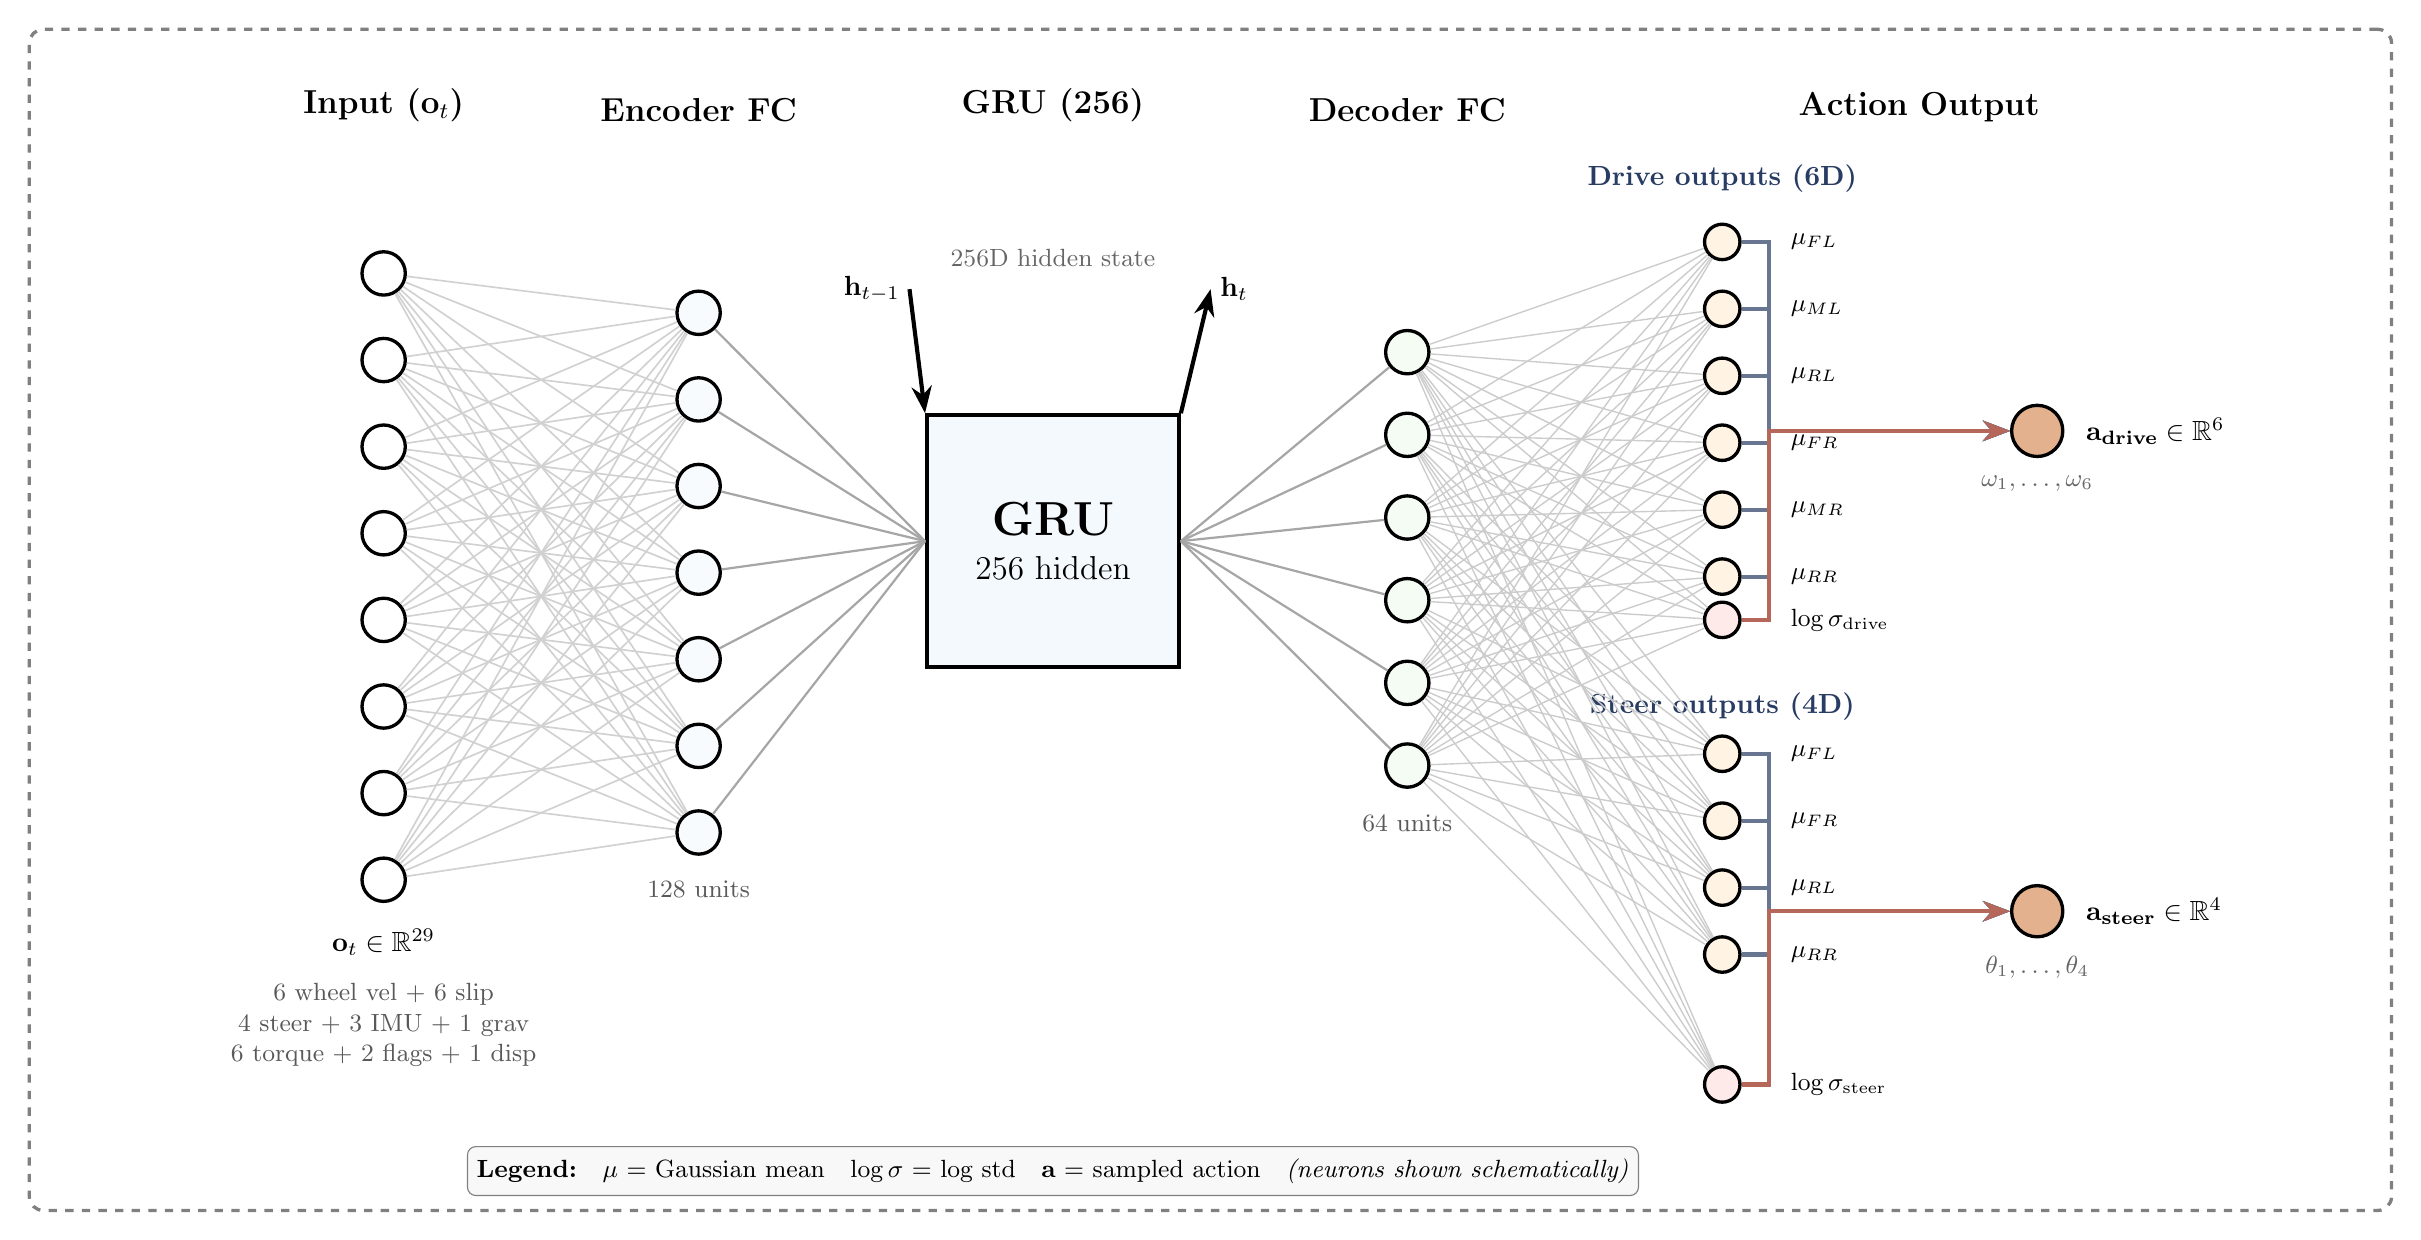
\begin{tikzpicture}[
      neuron/.style={circle, draw=black, line width=1.2pt,
                     minimum size=0.55cm, fill=white},
      grubox/.style={rectangle, draw=black, line width=1.4pt,
                     fill=lightblue!30, minimum width=3.2cm,
                     minimum height=3.2cm, align=center},
      arrow/.style={-Stealth, line width=1.5pt},
      dashedbox/.style={rectangle, draw=black!50, dashed,
                        line width=1.2pt, rounded corners=5pt},
    ]
      \node[dashedbox, minimum width=30cm, minimum height=15cm, fill=white]
            at (11.5, 0) {};
      %% Column headers
      \node[font=\large\bfseries, anchor=south] at ( 1.0, 6.2) {Input ($\mathbf{o}_t$)};
      \node[font=\large\bfseries, anchor=south] at ( 5.0, 6.2) {Encoder FC};
      \node[font=\large\bfseries, anchor=south] at ( 9.5, 6.2) {GRU (256)};
      \node[font=\large\bfseries, anchor=south] at (14.0, 6.2) {Decoder FC};
      \node[font=\large\bfseries, anchor=south] at (20.5, 6.2) {Action Output};
      %% Input neurons (8 representative for 29D)
      \foreach \i in {1,...,8}{
        \pgfmathsetmacro{\ypos}{4.4 - (\i-1)*1.1}
        \node[neuron] (in\i) at (1.0, \ypos) {};
      }
      \node[font=\normalsize\bfseries, below=0.2cm of in8]
            {$\mathbf{o}_t \in \mathbb{R}^{29}$};
      \node[font=\small, text=black!65, align=center, below=0.9cm of in8]{
        6 wheel vel $+$ 6 slip\\
        4 steer $+$ 3 IMU $+$ 1 grav\\
        6 torque $+$ 2 flags $+$ 1 disp};
      %% FC encoder (128 units)
      \foreach \i in {1,...,7}{
        \pgfmathsetmacro{\ypos}{3.9 - (\i-1)*1.1}
        \node[neuron, fill=lightblue!20] (fc1\i) at (5.0, \ypos) {};
      }
      \node[font=\small, text=black!65, below=0.2cm of fc17] {128 units};
      \foreach \i in {1,...,8}{
        \foreach \j in {1,...,7}{
          \draw[black!18, line width=0.6pt] (in\i) -- (fc1\j);
        }
      }
      %% GRU cell
      \node[grubox] (gru) at (9.5, 1.0) {\textbf{\LARGE GRU}\\[4pt]\large 256 hidden};
      \node[font=\normalsize\itshape] (ht_in)  at (7.2, 4.2) {$\mathbf{h}_{t-1}$};
      \node[font=\normalsize\itshape] (ht_out) at (11.8, 4.2) {$\mathbf{h}_{t}$};
      \draw[arrow] (ht_in.east)    -- (gru.north west);
      \draw[arrow] (gru.north east) -- (ht_out.west);
      \node[font=\small, text=black!60] at (9.5, 4.6) {256D hidden state};
      \foreach \i in {1,...,7}{
        \draw[black!35, line width=0.8pt] (fc1\i) -- (gru.west);
      }
      %% FC decoder (64 units)
      \foreach \i in {1,...,6}{
        \pgfmathsetmacro{\ypos}{3.4 - (\i-1)*1.05}
        \node[neuron, fill=lightgreen!30] (fc2\i) at (14.0, \ypos) {};
      }
      \node[font=\small, text=black!65, below=0.2cm of fc26] {64 units};
      \foreach \i in {1,...,6}{
        \draw[black!35, line width=0.8pt] (gru.east) -- (fc2\i);
      }
      %% Drive output head (6D)
      \node[font=\normalsize\bfseries, text=deepblue] at (18.0, 5.6)
            {Drive outputs (6D)};
      \foreach \i/\name in {1/FL, 2/ML, 3/RL, 4/FR, 5/MR, 6/RR}{
        \pgfmathsetmacro{\ypos}{4.8 - (\i-1)*0.85}
        \node[neuron, fill=lightorange!60, minimum size=0.45cm] (mu_d\i)
              at (18.0, \ypos) {};
        \node[font=\small, right=0.5cm of mu_d\i] {$\mu_{\name}$};
      }
      \node[neuron, fill=lightred!60, minimum size=0.45cm] (ls_d)
            at (18.0, 0.0) {};
      \node[font=\small, right=0.5cm of ls_d] {$\log\sigma_{\text{drive}}$};
      %% Steer output head (4D)
      \node[font=\normalsize\bfseries, text=deepblue] at (18.0, -1.1)
            {Steer outputs (4D)};
      \foreach \i/\name in {1/FL, 2/FR, 3/RL, 4/RR}{
        \pgfmathsetmacro{\ypos}{-1.7 - (\i-1)*0.85}
        \node[neuron, fill=lightorange!60, minimum size=0.45cm] (mu_s\i)
              at (18.0, \ypos) {};
        \node[font=\small, right=0.5cm of mu_s\i] {$\mu_{\name}$};
      }
      \node[neuron, fill=lightred!60, minimum size=0.45cm] (ls_s)
            at (18.0, -5.9) {};
      \node[font=\small, right=0.5cm of ls_s] {$\log\sigma_{\text{steer}}$};
      %% Sampled actions
      \node[neuron, fill=accentorange!50, minimum size=0.65cm]
            (a_d) at (22.0,  2.4) {};
      \node[font=\normalsize\bfseries, right=0.15cm of a_d]
            {$\mathbf{a}_{\text{drive}} \in \mathbb{R}^6$};
      \node[font=\small, text=black!60, below=0.1cm of a_d]
            {$\omega_1,\ldots,\omega_6$};
      \node[neuron, fill=accentorange!50, minimum size=0.65cm]
            (a_s) at (22.0, -3.7) {};
      \node[font=\normalsize\bfseries, right=0.15cm of a_s]
            {$\mathbf{a}_{\text{steer}} \in \mathbb{R}^4$};
      \node[font=\small, text=black!60, below=0.1cm of a_s]
            {$\theta_1,\ldots,\theta_4$};
      %% FC2 → output head connections
      \foreach \i in {1,...,6}{
        \foreach \j in {1,...,6}{ \draw[black!20, line width=0.5pt] (fc2\i) -- (mu_d\j);
        }
        \foreach \j in {1,...,4}{ \draw[black!20, line width=0.5pt] (fc2\i) -- (mu_s\j);
        }
        \draw[black!20, line width=0.5pt] (fc2\i) -- (ls_d);
        \draw[black!20, line width=0.5pt] (fc2\i) -- (ls_s);
      }
      %% Output → action arrows
      \foreach \i in {1,...,6}{
        \draw[arrow, color=deepblue!70] (mu_d\i.east) -- ++(0.35,0) |- (a_d.west);
      }
      \draw[arrow, color=marsred!70] (ls_d.east) -- ++(0.35,0) |- (a_d.west);
      \foreach \i in {1,...,4}{
        \draw[arrow, color=deepblue!70] (mu_s\i.east) -- ++(0.35,0) |- (a_s.west);
      }
      \draw[arrow, color=marsred!70] (ls_s.east) -- ++(0.35,0) |- (a_s.west);
      %% Legend
      \node[draw=black!50, fill=boxgray, rounded corners=3pt,
            align=left, font=\small] at (9.5, -7.0) {%
        \begin{tabular}{@{}l@{}}
          \textbf{Legend:}\quad
          $\mu$ = Gaussian mean\quad
          $\log\sigma$ = log std\quad
          $\mathbf{a}$ = sampled action\quad
          \textit{(neurons shown schematically)}
        \end{tabular}};
    \end{tikzpicture}%
  }
  \caption{GRU-PPO recurrent actor network. The 29D proprioceptive observation is
    encoded by a 128-unit fully connected layer, passed through a 256-unit GRU that
    maintains entrapment history $\mathbf{h}_t$, then decoded by a 64-unit FC layer
    to a 10D Gaussian policy: 6D drive velocities and 4D steer angles. The
    asymmetric critic has an identical architecture but reads the full 37D
    observation (policy obs~$||$~8 privileged features); only the actor's 29D slice
    is exported to ONNX for deployment.}
  \label{fig:policy_arch}
\end{figure*}

% ══════════════════════════════════════════════════════════════
\section{Algorithms}
\label{sec:algorithms}

Algorithm~\ref{alg:detection} describes the dual-mode online entrapment detection
used during both training and deployment. Algorithm~\ref{alg:training} presents the full curriculum PPO-GRU training
procedure with GAE advantage estimation~\cite{schulman2015gae}.

\begin{algorithm}[t]
  \caption{Dual-Mode Entrapment Detection}
  \label{alg:detection}
  \begin{algorithmic}[1]
    \Require Wheel angular vel.\ $\boldsymbol{\omega}$, linear vel.\ $v_x$,
             drive torques $\boldsymbol{\tau}$, previous torques
             $\boldsymbol{\tau}_\text{prev}$
    \Ensure  Entrapment flag $f_\text{ent}$, anomaly flag $f_\text{anom}$

    \State \textbf{// --- Slip ratio ---}
    \For{$i = 1 \to 6$}
      \State $\sigma_i \gets 1 - v_{\text{lin},i} / (\omega_i \cdot r)$
    \EndFor
    
    \State $\bar{\sigma} \gets \tfrac{1}{6}\sum_i \sigma_i$

    \State \textbf{// --- Entrapment counter ---}
    \If{$|v_x| < 0.15$ \textbf{and} $\bar{\sigma} > 0.4$}
      \State $c_\text{ent} \gets c_\text{ent} + 1$
    \Else
      \State $c_\text{ent} \gets 0$
    \EndIf
    \State $f_\text{ent} \gets (c_\text{ent} \geq 15)$

    \State \textbf{// --- Torque anomaly counter (OR logic + leaky) ---}
    \State $\bar{\tau}_n     \gets \tfrac{1}{6}\sum_i|\tau_i|/\tau_\text{max}$
    \State $\Delta\bar{\tau} \gets |\bar{\tau}_n - \bar{\tau}_{n,\text{prev}}|$
    \If{$\bar{\tau}_n > 0.85$ \textbf{or} $\Delta\bar{\tau} > 0.10$}
      \State $c_\text{anom} \gets \min(c_\text{anom} + 1,\; 30)$
  
    \Else
      \State $c_\text{anom} \gets \max(c_\text{anom} - 0.5,\; 0)$
        \Comment{leaky decay}
    \EndIf
    \State $f_\text{anom} \gets (c_\text{anom} \geq 20)$

    \State \Return $f_\text{ent},\; f_\text{anom}$
  \end{algorithmic}
\end{algorithm}

\begin{algorithm}[t]
  \caption{Curriculum PPO-GRU Training for Entrapment Recovery}
  \label{alg:training}
  \begin{algorithmic}[1]
    \Require $N{=}32$ envs, $T{=}200\,000$ steps, rollout $L{=}64$,
             BPTT length~32, progress $p{\in}[0,1]$,
             clip $\epsilon{=}0.2$, $\alpha{=}0.03$, GRU hidden~256

    \State Initialise $\pi_\theta$ (actor, 29D input),
           $V_\phi$ (critic, 37D input); $\mathbf{h}^{(i)}_0 \gets \mathbf{0}$ $\forall i$

    \For{$t = 0$ \textbf{to} $T$ \textbf{step} $L$}

      \State \textbf{// --- Rollout ---}
      \For{each env $i$, each step $\ell = 0 \ldots L{-}1$}
        \State Sample $\phi_\text{esc}^{(i)} \sim \mathcal{U}(0,2\pi)$
               on episode reset
        \State $\mathbf{o}^{(i)} \gets \text{GetObs}(i)$\quad
               (37D: 29D policy + 8D privileged)
 
        \State $f_\text{ent}^{(i)}, f_\text{anom}^{(i)} \gets$
               Alg.\,\ref{alg:detection}
        \State $\mathbf{a}^{(i)}, \mathbf{h}^{(i)} \gets
               \pi_\theta(\mathbf{o}^{(i)}_{[:29]}, \mathbf{h}^{(i)})$
        \State Apply $\mathbf{a}^{(i)}$; step MPM + MuJoCo
        \State $r^{(i)} \gets$ Eq.\,\eqref{eq:reward}
      \EndFor

      \State \textbf{// --- PPO update ---}
      \State Compute GAE $\hat{A}_t$ ($\gamma{=}0.99$, $\lambda{=}0.95$)
      \For{epoch $= 1 \to 3$}
        \For{each mini-batch (8 per epoch)}
          \State $\rho_t \gets
                 \pi_\theta(a|o_{[:29]})/\pi_{\theta_\text{old}}(a|o_{[:29]})$
       
          \State $\mathcal{L} \gets
                 {-}\mathbb{E}\bigl[\min(\rho_t\hat{A},\;
                 \text{clip}(\rho_t,1{\pm}\epsilon)\hat{A})\bigr]$
                 $+ c_1(V_\phi - \hat{V})^2 - \alpha\mathcal{H}[\pi_\theta]$
          \State Update $\theta, \phi$ via Adam on $\mathcal{L}$
        \EndFor
      \EndFor

      \State \textbf{// --- Competence-gated curriculum ---}
      \State rate $\gets$ fraction of envs reaching 0.5\,m milestone
      \If{rate $> 0.40$ \textbf{and} $p < 1$}
        \State $p \gets \min(p + \Delta p,\,1)$
          \Comment{advance to deeper sinkage}
      \EndIf

    \EndFor
    \State \Return $\pi_\theta$
  \end{algorithmic}
\end{algorithm}

\FloatBarrier
% ══════════════════════════════════════════════════════════════
\section{Experimental Results}
\label{sec:results}

\subsection{Training Setup}

Training runs on a single workstation (NVIDIA RTX 5070\,Ti 16\,GB,
Intel i7) for 200\,000 timesteps across 32 parallel environments. Each environment contains ${\sim}150\,000$ MPM particles.
Policy frequency is 25\,Hz; physics runs at 50\,Hz (decimation~2,
4 MuJoCo substeps).

\subsection{Training Convergence}

The episodic return rises steadily as the competence-gated curriculum drives the
minimum sinkage toward the 28\,cm deep-burial ceiling. Policy entropy remains
above $0.5$\,nats throughout training, confirming no premature convergence to a
deterministic policy. Fig.~\ref{fig:training_convergence} shows the full
convergence picture.

\begin{figure}[t]
  \centering
  
\includegraphics[width=\linewidth]{training_overview.png}
  \caption{Episodic reward, escape rate, and policy entropy over 200\,k
    timesteps. Vertical dashed lines mark curriculum stage transitions.
    Entropy remains above 0.5\,nats throughout, confirming no collapse.}
  \label{fig:training_convergence}
\end{figure}

\begin{figure}[t]
  \centering
  
\includegraphics[width=\linewidth]{ppo_gru_regolith_reward_dual_axis.png}
  \caption{Reward and escape rate on dual axes. The escape rate (right axis)
    correlates with reward growth, validating that the reward function faithfully
    proxies escape success.}
  \label{fig:dual_axis}
\end{figure}

\subsection{Escape Performance}

\begin{table}[t]
  \centering
  \caption{Escape performance (200\,k timesteps, 32 envs). All values are
    mean$\,\pm\,$std over the final 10\,k training steps. \emph{Pending:} to be
    populated from the completed training run.}
  \label{tab:results}
  \renewcommand{\arraystretch}{1.2}
  \begin{tabular}{@{}lcc@{}}
    \toprule
    \textbf{Metric} & \textbf{Value} & \textbf{Note} \\
    \midrule
    Overall escape rate (3.0\,m) & \textit{pending} & Full curriculum \\
    Milestone 0.5\,m rate        & \textit{pending} & End of training \\
    Milestone 1.0\,m rate        & \textit{pending} & End of training \\
    Milestone 2.0\,m rate       
    & \textit{pending} & End of training \\
    Milestone 3.0\,m rate        & \textit{pending} & End of training \\
    Mean time to escape (steps)  & \textit{pending} & 25\,Hz policy \\
    Mean episode reward          & \textit{pending} & Final 10\,k steps \\
    Curriculum progress $p$      & $\to 1$           & Continuous advance \\
    \bottomrule
  \end{tabular}
\end{table}

\begin{figure}[t]
  
  \centering
  
\includegraphics[width=\linewidth]{escape_rate.png}
  \caption{Milestone completion rates (0.5, 1.0, 2.0, 3.0\,m) over training. The 0.5\,m rate crossing 40\% drives the competence-gated curriculum
    toward deeper sinkage.}
  \label{fig:escape_rate}
\end{figure}

\subsection{Reward Component Analysis}

\begin{figure}[t]
  \centering
  
\includegraphics[width=\linewidth]{reward_breakdown.png}
  \caption{Per-term reward contribution over training. The escape bonus
    ($w{=}20$) dominates early; rocking ($w{=}5$) and progress ($w{=}1.5$)
    grow as the policy develops complete escape strategies.}
  \label{fig:reward_breakdown}
\end{figure}

The escape bonus (weight~20) dominates during early training when the rover is
consistently entrapped. As escape skill develops, the rocking term (weight~5)
contributes increasingly during the pre-escape phase, and the progress term
carries the final 0.5\,m to the 3.0\,m milestone. The absence of catastrophic
forgetting across curriculum stage transitions validates the reward design.

\subsection{Policy Metrics and Emergent Behaviours}

\begin{figure}[t]
  \centering
  
\includegraphics[width=\linewidth]{policy_metrics.png}
  \caption{Policy metrics over training: action smoothness
    ($\|\Delta\mathbf{a}\|$) and GRU hidden state norm. Smoothness improves as
    the policy learns deliberate escape manoeuvres over high-frequency jitter.}
  \label{fig:policy_metrics}
\end{figure}

The policy develops qualitatively distinct strategies by entrapment severity:

\textbf{Shallow ($d < 15$\,cm):} Rapid forward surge with all drive wheels at
maximum and front steering angled outward, bulldozing clear in 3--5 steps. \textbf{Deep ($d \geq 20$\,cm):} Coordinated rocking---alternating forward/reverse
drive commands with oscillating steer angles---progressively loosening soil before
a sustained escape. This behaviour emerges solely from the $r_\text{rock}$
incentive and was not explicitly scripted. \textbf{Asymmetric sinkage:} Differential torque---higher drive on the less-buried
side, reverse steer on the buried side---pivots the rover out of the entrapment
zone at a slight heading angle. \FloatBarrier
% ══════════════════════════════════════════════════════════════
\section{Sim-to-Sim Navigation Validation}
\label{sec:sim2sim}

We validate the complete dual-brain system in a sim-to-sim A$\to$B navigation
scenario: the rover starts at point A, must reach goal B, and an MPM sand patch
is placed across the shortest path to force entrapment. This tests the full
hierarchy: navigation, detection, recovery, and re-planning.

\subsection{Dual-Brain Architecture}

The on-board hierarchy comprises three layers (Fig.~\ref{fig:dual_brain}):

\textbf{Layer 1 --- PD Navigation.}
A proportional-derivative waypoint follower drives the rover toward the GPS
goal B. Heading error drives the four steering joints; all six drive wheels
run at constant speed. The navigation brain has no knowledge of sand patches. \textbf{Layer 2 --- Entrapment Detection.}
The dual-mode detector (Eq.~\eqref{eq:entrapment}--\eqref{eq:anomaly})
monitors $f_\text{ent}$ continuously. When $f_\text{ent}$ fires for 15
consecutive steps, control transfers to the Escape Brain. \textbf{Layer 3 --- Recovery.}
The trained GRU-PPO policy takes over. The escape direction is set to
$\hat{\mathbf{e}}_\text{deploy}$ (GPS bearing toward B) via the
zero-shot generalisation property. Recovery is declared when the projected
displacement along $\hat{\mathbf{e}}$ exceeds 3.0\,m. Control returns
to Layer~1 immediately. \begin{figure}[t]
  \centering
  \resizebox{0.88\linewidth}{!}{%
    \begin{tikzpicture}[
      >=Stealth, font=\sffamily\small,
      sbox/.style={rectangle, draw=black!50, thick, rounded corners=3pt,
                   fill=white, align=center, minimum width=2.9cm,
                   minimum height=1.1cm},
      dbox/.style={rectangle, draw=black!60, line width=1.2pt,
                   rounded corners=4pt, fill=white, align=center,
  
                   minimum width=9.8cm, minimum height=1.5cm},
      nbox/.style={rectangle, draw=black!60, line width=1.2pt,
                   rounded corners=4pt, fill=white, align=center,
                   minimum width=3.9cm, minimum height=1.6cm},
      ebox/.style={rectangle, draw=black!60, line width=1.2pt,
                  
                   rounded corners=4pt, fill=lightblue!30, align=center,
                   minimum width=3.9cm, minimum height=1.6cm},
      mbox/.style={rectangle, draw=black!55, line width=1.2pt,
                   rounded corners=4pt, fill=white, align=center,
                   minimum width=5.5cm, minimum height=1.1cm},
      dec/.style={diamond, draw=orange!65!black, line width=1.2pt,
            
                   fill=none, align=center, aspect=2.8,
                  font=\small\bfseries},
      a/.style={-Stealth, thick},
      ga/.style={-Stealth, line width=1.5pt, color=AccentGreen!80!black},
      ra/.style={-Stealth, line width=1.5pt, color=MarsRust!80!black},
      da/.style={-Stealth, thick, dashed, color=black!35},
    ]
      \node[rectangle, draw=black!45, thick, rounded corners=8pt, dashed,
            fill=none, minimum width=14.0cm, minimum height=10.4cm]
         
            (rpi) at (0, 1.6) {};
      \node[anchor=north west, font=\footnotesize, text=black!50]
            at (rpi.north west) {Onboard Computer (RPi\,5)};
      \node[sbox] (imu) at (-4,  5.6) {\textbf{IMU}\\{\scriptsize acc, gyro}};
      \node[sbox] (enc) at ( 0,  5.6) {\textbf{Wheel Encoders}\\
                                       {\scriptsize vel, torque}};
      \node[sbox] (gps) at ( 4,  5.6) {\textbf{Goal / GPS}\\
                                       {\scriptsize target position}};
      \node[dbox] (det) at (0, 3.6) {%
        \textbf{Dual-Mode Entrapment Detector}\\[2pt]
        {\small Slip-ratio counter + Torque anomaly (Alg.\,1)}\\
        {\scriptsize $f_\text{ent}$, $f_\text{anom}$}};
      \node[dec] (dmd) at (0, 1.7) {\textbf{Entrapped?}};

      \node[nbox] (nav) at (-4, -0.3) {%
        \textbf{Navigation Brain}\\[2pt]
        {\small PD Waypoint Follower}\\
        {\scriptsize GPS $\to$ motor commands}};
      \node[ebox] (esc) at (4, -0.3) {%
        \textbf{Escape Brain}\\[2pt]
        {\small GRU-PPO (our work)}\\
        {\scriptsize $\hat{\mathbf{e}} = $ GPS dir to B}};
      \node[mbox] (mot) at (0, -2.6) {%
        \textbf{Motor Commands}\\{\scriptsize drive (6) + steer (4)}};
      \draw[a]  (imu.south) -- (imu|-det.north);
      \draw[a]  (enc.south) -- (det.north);
      \draw[a]  (gps.south) -- (gps|-det.north);
      \draw[a]  (det.south) -- (dmd.north)
                node[midway, right=4pt, font=\scriptsize] {entrap flag};
      \draw[ga] (dmd.west)  -| (nav.north)
                node[pos=0.18, above, font=\small\bfseries,
                     text=AccentGreen!80!black] {No};
      \draw[ra] (dmd.east)  -| (esc.north)
                node[pos=0.18, above, font=\small\bfseries,
                     text=MarsRust] {Yes};
      \draw[ga] (nav.south) |- (mot.west);
      \draw[ra] (esc.south) |- (mot.east);
      \draw[da] (esc.west)  -- (0,-0.3) -- (dmd.south)
                node[pos=0.75, right=3pt, font=\scriptsize,
                     text=black!45] {escaped};
    \end{tikzpicture}%
  }
  \caption{Dual-brain on-board architecture. During normal traversal the PD
    Navigation Brain drives toward GPS goal B; the dual-mode entrapment detector
    triggers handover to the GRU-PPO Escape Brain when $f_\text{ent}$ fires. Escape direction is set to the GPS bearing toward B (zero-shot
    generalisation). After escape, control returns to navigation automatically.}
  \label{fig:dual_brain}
\end{figure}

\subsection{Experimental Protocol}

20 trials per condition; 8 parallel environments; fixed seed (123) for
identical sand placement across conditions. Goal B is placed 6\,m ahead of
start A; the sand patch intercepts the straight-line path at 2\,m.
Max episode length: 2\,000 policy steps (80\,s at 25\,Hz). \textbf{Conditions:}
\begin{itemize}
  \item \textbf{Recovery} (ours): dual-brain with escape primitive activated.
  \item \textbf{Baseline}: PD navigation only, escape primitive disabled; rover
        drives until timeout after entrapment.
\end{itemize}

\begin{table}[t]
  \centering
  \caption{Sim-to-sim A$\to$B navigation validation (20 trials per condition).
    Mean~$\pm$~std. \emph{Pending}: to be populated after training completes.}
  \label{tab:sim2sim}
  \renewcommand{\arraystretch}{1.2}
  \begin{tabular}{@{}lcc@{}}
    \toprule
    \textbf{Metric} & \textbf{Baseline (no recovery)}
                    & \textbf{Ours (with recovery)} \\
    \midrule
    Goal reach rate (\%)       & \textit{pending} & \textit{pending} \\
    Recovery rate (\%)         & ---              
    & \textit{pending} \\
    Time to escape (steps)     & ---              & \textit{pending} \\
    Time to goal (steps)       & \textit{pending} & \textit{pending} \\
    Path efficiency            & \textit{pending} & \textit{pending} \\
    Escape heading error (deg) & ---              & \textit{pending} \\
    \bottomrule
 
  \end{tabular}
\end{table}

\subsection{Expected Outcomes}

The baseline is expected to show near-zero goal-reach rate: the PD controller
has no mechanism to escape once $f_\text{ent}$ fires, so the episode exhausts
its step budget with the rover stationary inside the sand patch. The recovery
condition is expected to show high escape rate and substantially higher goal-reach
rate, quantifying the value of the autonomous recovery primitive. Path efficiency
below 1.0 is expected due to the heading deviation induced by the rocking manoeuvre;
the escape heading error (angle between $\hat{\mathbf{e}}_\text{deploy}$ and the
final escape direction) validates the zero-shot GPS-direction generalisation. % ══════════════════════════════════════════════════════════════
\section{Discussion}
\label{sec:discussion}

\subsection{Why MPM is Necessary for Entrapment Recovery}

Rigid terrain approximations cannot capture the temporal dynamics of granular
entrapment: in MPM, soil flows, compacts, and redistributes under wheel loading
over multiple seconds. This is precisely the signal the GRU hidden state must
track. The rocking behaviour is physically meaningful only in this context---each
oscillation loosens surrounding particles incrementally. A policy trained in
rigid terrain cannot exploit this phenomenon, since the soil state does not
evolve. The absence of MPM would force the policy to learn a purely kinematic
recovery strategy, which fails in the presence of variable sinkage depth. \subsection{Comparison with Bi \& Ding (2026)}

Compared to Bi \& Ding~\cite{bi2026escape}, our system addresses a strictly
harder problem: 6-wheel rocker-bogie kinematics, 10D action space, granular
sinkage (vs.~rigid terrain lift-off), Mars gravity (62\% lower traction), and no
expert demonstrations. Their reported 90\% success is obtained at 4\,M steps in
a rigid-terrain setting; our escape rate (Table~\ref{tab:results}) is measured
after 200\,k steps in full MPM coupling. Additionally, our omnidirectional
training enables zero-shot goal-directed recovery, a capability absent from prior
work. \subsection{Limitations}

The primary limitation is the absence of direct cross-engine validation; mitigated by the sim-to-sim A$\to$B scenario using the same physics engine but
a fundamentally different task structure (navigation + detection + recovery +
re-planning). Domain randomisation over motor gains and sensor noise
following~\cite{tobin2017domainrand,andrychowicz2020learning} is planned for
future work to improve physical transfer robustness. Hardware deployment on the
AAU rover is contingent on hardware availability. % ══════════════════════════════════════════════════════════════
\section{Future Work}
\label{sec:future}

\begin{itemize}
  \item \textbf{Extended training}: scale to 500\,k--1\,M timesteps and 64+
        environments on a multi-GPU cluster to close the sample-efficiency gap
        with~\cite{bi2026escape}.
  \item \textbf{Physical deployment}: export actor to ONNX; run at ${\geq}10$\,Hz
        on Raspberry Pi~5; validate on the AAU Mars rover hardware in a sand pit.
  \item \textbf{CNN-GRU sinkage classifier}: Phase~2 classifier trained on
        auto-labelled simulator ground-truth, replacing the threshold-based
        detector with a learned probabilistic model.
  \item \textbf{Ablation studies}: GRU vs.\ MLP policy, asymmetric critic on/off,
        omnidirectional training vs.\ fixed-heading, to quantify each design
        choice's contribution.
  \item \textbf{Terrain diversity}: rock obstacles, slopes up to~$15^\circ$, and
        mixed granular--rocky terrain within the same episode.
\end{itemize}

\FloatBarrier
% ══════════════════════════════════════════════════════════════
\section{Conclusion}
\label{sec:conclusion}

We presented the first DRL-based entrapment recovery system coupling Newton MPM
granular physics with MuJoCo rigid-body dynamics inside Isaac Lab for a 6-wheel
rocker-bogie Mars rover under Mars gravity. A PPO+GRU recurrent policy trained
with competence-gated curriculum sinkage scheduling and an 8-term shaped reward
produces emergent rocking and asymmetric steering behaviours not explicitly
programmed. The asymmetric actor-critic (29D actor, 37D privileged critic) and
dual-mode entrapment detector (slip-ratio + torque anomaly with leaky OR logic)
together provide a ${\approx}0.6$\,s early-warning advantage over the ground-truth
flag. Omnidirectional escape training---per-episode $\mathcal{U}(0,2\pi)$ heading
sampling---enables zero-shot GPS-directed recovery at deployment without any
heading-specific fine-tuning, validated in a sim-to-sim A$\to$B navigation
scenario against a no-recovery baseline (Table~\ref{tab:sim2sim}). The Newton MPM
coupling is both the key technical contribution and the essential physical
ingredient: without granular simulation, the temporal sinkage dynamics that
necessitate a recurrent policy cannot be faithfully modelled. \FloatBarrier
\balance
\bibliographystyle{unsrt}
\bibliography{references}

\end{document}
